\documentclass[a4paper,12pt]{article}
\usepackage[utf8]{inputenc}

%\title{Coupled Excitations in the Benzene Dimer}
%\author{Thomas Konincks}
%\date{December 2013 - June 2014}

\usepackage{natbib} %?
\usepackage{graphicx} %?
\usepackage{subfigure} %subfigures in figures
\usepackage{textcomp} %?
\usepackage{amsmath} %mathematics package
\usepackage{nicefrac} %to use \nicefrac{}{}
\usepackage{geometry} %to reduce the margin
\usepackage{microtype} %?
\usepackage[superscript,biblabel]{cite} %superscript refernces
\usepackage{hyperref} %clickable refrences and summary
\usepackage[font={it}]{caption} %italic captions for the pictures
\usepackage{eso-pic} %for the background picture of the title page
\usepackage{transparent} %for the opacity of the pictures

\newcommand{\jline}{\vspace{10pt}}
\newcommand{\ang}{\mbox{\normalfont\AA \,}}
\newcommand{\etal}{\textit{et al.}}

%\newcommand\BackgroundPic{%
%\put(0,0){%
%\parbox[b][\paperheight]{\paperwidth}{%
%\vfill
%\centering
%\transparent{0.2}
%\includegraphics[width=\paperwidth,height=\paperheight,
%keepaspectratio]{pics/bD_fde.png}%
%\vfill
%}}}

%\geometry{scale=0.8, nohead} %smaller margins
%\setlength{\footskip}{50pt}

\begin{document}

%\maketitle

%\AddToShipoutPicture*{\BackgroundPic}

\begin{titlepage}
    \centering
    \vfill
    {\bf{\Huge
    Dynamics of Fluids\\in\\Random Environments
    \vfill
    \LARGE
    Thomas Konincks
    \vskip1cm
    Master Theoretical Chemistry and Computational Modeling
    \vfill
    \LARGE September 2014}}    
    \vfill
    
\includegraphics[height=1.8cm]{logos/logo_rug.png}
\end{titlepage}

\newpage

\tableofcontents

\section{Introduction}

In the recent few years, porous materials have attracted much attention, especially because of the possibility of hydrogen storage, for which the MOF materials are the most viewed \cite{Yan2009}. MOFs are an example of a porous solid that presents a very high symmetry, due to their crystalline structure. However in this work we will be concerned with an other type of porous medium: the disordered porous materials (i.e. without any symmetry or long distance order), with randomly arranged pores.\jline

This type of materials contains most of the natural porous systems: some rocks are known to be porous (sand, gravel and volcanic rocks for example), the soil has also some degree of porosity that is extensively studied in order to make good use of natural resources, and understand geological phenomenons \cite{Nasta2009, Grosbellet2011, Gab2014, Walczak2006}. But porosity can also be wanted, created and controlled: the controlled porous glasses are a good example, as well as the novel aerogel materials that present an exceptionally high degree of porosity.\jline

Dynamics of liquids in confined disordered environment is a kind of system that is difficult to capture experimentally, because of the speed of the dynamics and the fact that the system is by definition confined. Some experiments have given some interesting results on comparable systems, but the main way to study them is to develop models that are able to compute information on their dynamics. Experimentally or theoretically, there are essentially two phenomenas that people want to capture:

\begin{itemize}

\item First, the liquid-glass transition. If the dynamics are slow enough (i.e. the potential in which the particle moves: the matrix), the system will undergo a phase transition, meaning that the colloids will be completely trapped inside the potential and the dynamics stopped. The glass phase is simply a liquid which dynamics are "frozen".\jline

\item The second phenomenon that has been observed in this kind of confined environments is the three step relaxation that is characteristic of supercooled liquids. High temperature and non confined fluids follows a simple relaxation scheme as shown in fig. \ref{relaxations} (left): when the time increases, the system goes smoothly from a non-relaxed state to a state where all the distances have been balanced, and the potential energy minimized. For confined fluids, the relaxation is done in three steps: one first simple relaxation (I) that follows the usual dynamics of the fluids (as for the non-confined case) where the particles explore their local minima, the second step (II): a plateau and a second relaxation during which the particles appear trapped in the cages formed by the matrix of the solid, this step is called the $\alpha$ relaxation regime. The third step is the $\beta$ relaxation regime, a very slow approach towards the long time diffusion regime, during which the particles will be able to hop from a site to another, their dynamics can then be compared to a random walk from site to site.\jline
\end{itemize}

\begin{figure}[htbp]
\centering
\subfigure
{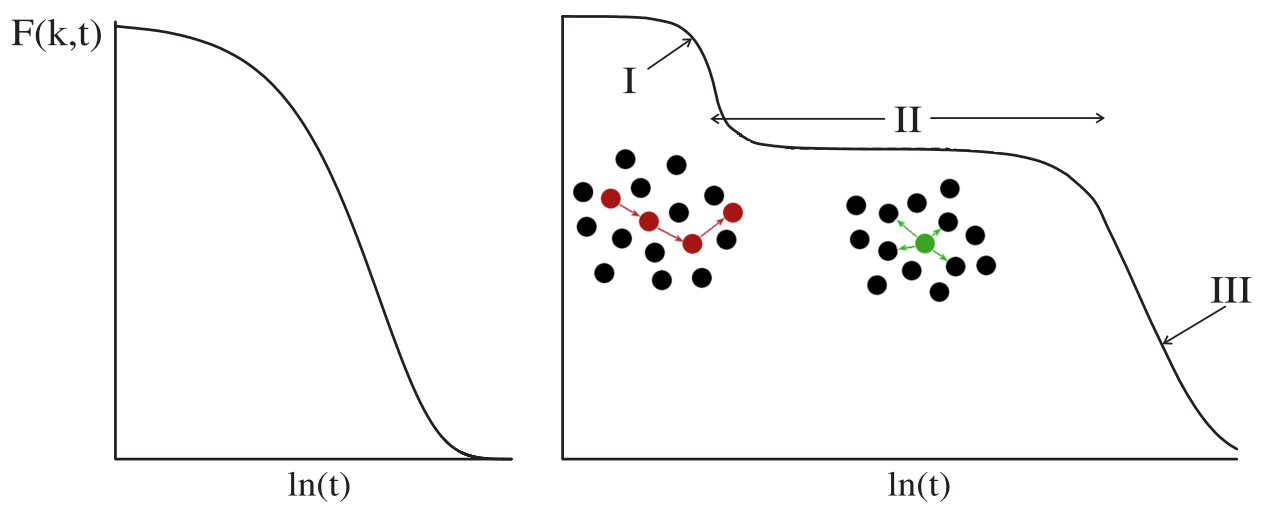
\includegraphics[width=14cm]{pics/relaxations.png}}
\caption{Left: Exponential decay for a normal liquid. Right: supercooled liquids do not have such a simple decay. Notice the logarithmic scale. D. Reichman and P. Charbonneau, J. Stat. Mech.: Theory and Experiment, \textbf{05}, P05013 (2005).}
\label{relaxations}
\end{figure}

Studying the dynamics of fluids in disordered environments allows to make predictions on various types of systems such as supercooled liquid \cite{} or glasses \cite{}, but also as living cells \cite{} or protein foldings \cite{}.\jline

Section \ref{theory} will make a summary of the different theories and models that have been developed in order to understand and make predictions on the dynamics and the phase transitions that these trapped system undergo. A special emphasis will be put on the mode-coupling theory that is to this date the most efficient theory, and one that has made the most accurate predictions.
The next section will present some of the experimental works that have been made in the field.\jline

\section{Experimental works}
\label{exp}

Having experimental evidence of phenomenas that happen at the microscopic level, confined into a porous material is very difficult, not to say impossible. However scientists have found ways to observe macroscopic phenomena that have the exact same behaviour than molecules inside a porous matrix. The experiments have been made in one, then in two dimensions. Statistical mechanics is one of the few fields in which the validity of the experiments have to be compared to theory, and not the opposite. Thus, each of the experiments have been "dubbed" with a Monte-Carlo simulation to compare the results (see sec. \ref{monte-carlo}).

\subsection{Dynamics of colloids in dimensional random optic potential}

The diffusion of particles in a disordered environment can be seen as a diffusion of those particles in an potential energy landscape, that has a finite value if the pores are not permanent, or goes to infinity when the particles touches edges of pores in a hard matrix. Some colloids are known to have an interaction with light, either attractive or repulsive (this force is lead by the difference of refractive index, higher or lower than that of the environment, leads to respectively an attractive or a repulsive force).\jline

That observation has lead Hanes \etal \cite{Hanes2012} to conduct an experiment in which they let polystyrene colloids suspended in heavy water (D$_2$O) flow in a channel. The channel is then randomly hit by laser beams that creates a one dimensional random potential that the particles feels.\\
An other experiment, made by Evers \etal \cite{Evers2013} focused on a two dimensional description of the dynamical phenomenons. Instead of letting the colloids flow in a channel, they sent a random light interference figure (called speckle) on polystyrene particles floating in heavy water (as argued vy Evers \etal the heavy water allows the particles to cream rather than sediment). The speckle simulates the random arrangement of a physical matrix. The experiment has simply been extended to one more dimension compared to the one of Hanes \etal.\jline

Fig. \ref{potential and colloids} (left) shows a potential that was used by Evers \etal to make a Monte-Carlo simulation in order to complete their experimental work (see sec. \ref{monte-carlo}). The potential is supposed to be very close to the potential that their produced experimentally. It clearly  presents maximas, minimas and saddle points. Knowing that the colloids have a repulsive interaction with light, they will tend to stay at the minimas and avoid the maximas. The colloids will however be able to hop from one minima to another if the energy barrier is low (i.e. saddle points are low) enough or if the colloids are fast (i.e. the temperature is high) enough.\jline

Fig. \ref{potential and colloids} (right) shows a picture of the trajectories of the colloids in the system studied by Evers \etal. The picture is taken with a CMOS camera (usual camera). We can see that the colloids that are trapped inside the speckle (green circle) do not move as much as the colloids outside the speckle do, which can freely explore all the space available to them. The particles inside the speckle remain trapped for a more or less long time inside the minimas of the potential, sometimes hopping from a minima to the other (that behaviour can be compared to a random walk, see sec.\ref{random walk}). The presence of the random potential slows down the dynamics of the system drastically.\jline

\begin{figure}[htbp]
\centering
\subfigure
{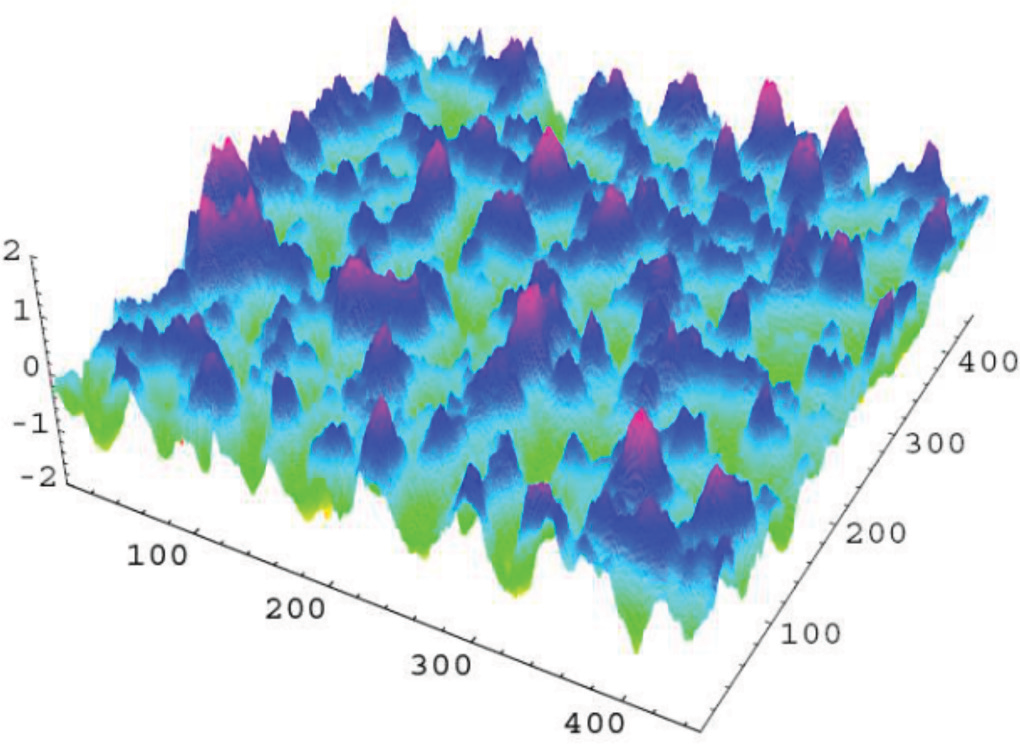
\includegraphics[width=7cm]{pics/optic_pot.png}}
\subfigure
{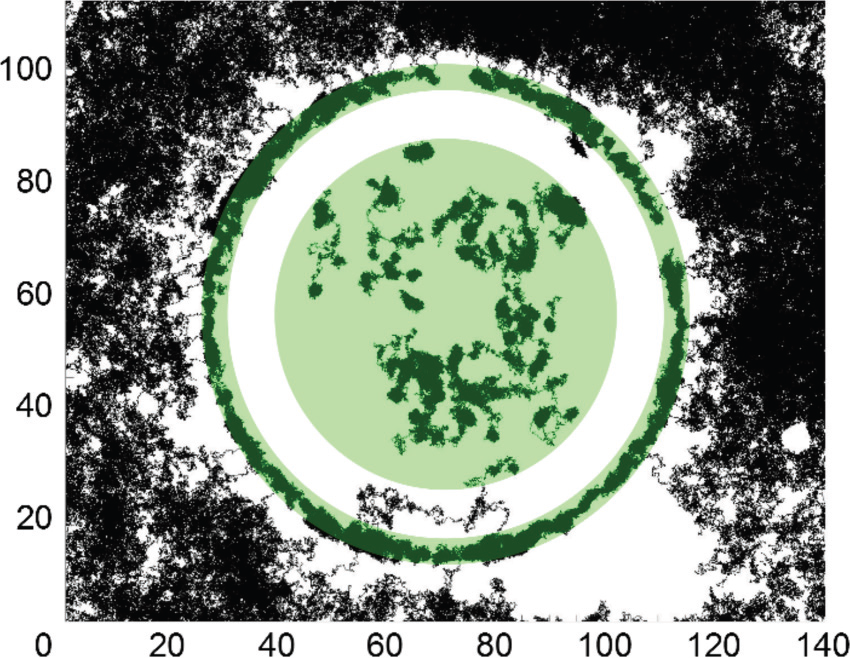
\includegraphics[width=7cm]{pics/colloids.png}}
\caption{(left) Potential generated for a Monte-Carlo simulation, it is suppose to reflect the potential felt by the colloids beamed by a laser speckle.\\(right) Trajectories of particles undergoing diffusion in a two-dimensional plane, part of which contains a random potential (green background), which is separated by a barrier (white/green rings) from the surroundings (white background).\\ \small F. Evers \etal, Physical Review E, \textbf{88}, 022125 (2013)}
\label{potential and colloids}
\end{figure}

Fig. \ref{msd ndc  exp} shows the mean square displacement and the normalized diffusion coefficient for the experiment conducted by Hanes \etal (left) and the experiment by Evers \etal. The mean square displacement measures how much the particles have moved from their initial position in function of time, it is calculated as:

\begin{equation}
\left< \Delta r(t)^2\right> = \sum_{i=1}^d \left< x_i(t)^2 \right>  - \left< x_i(t) \right>^2
\end{equation}

The normalized diffusion coefficient:

\begin{equation}
\frac{D(t)}{D_0}=\frac{1}{2dD_0}\frac{d}{dt}\left< \Delta r(t)^2 \right>
\end{equation}

In both equations, d is the dimension and the $\left< \hdots \right>$ represents the time average.

\begin{figure}[htbp]
\centering
\subfigure
{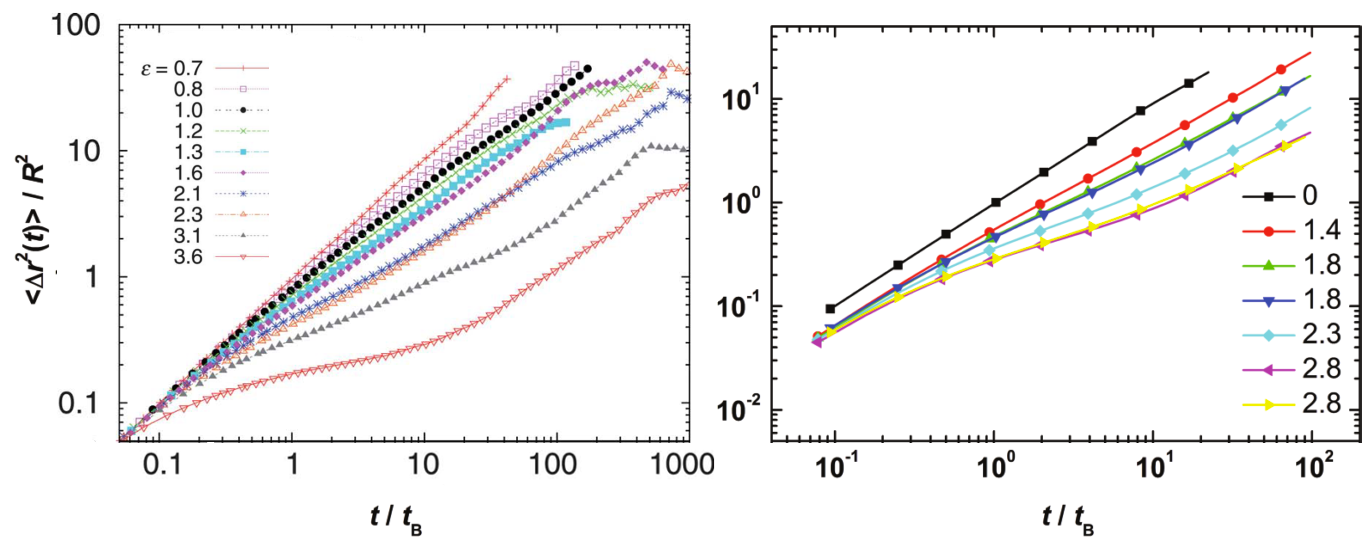
\includegraphics[width=14cm]{pics/msd_exp.png}}
\subfigure
{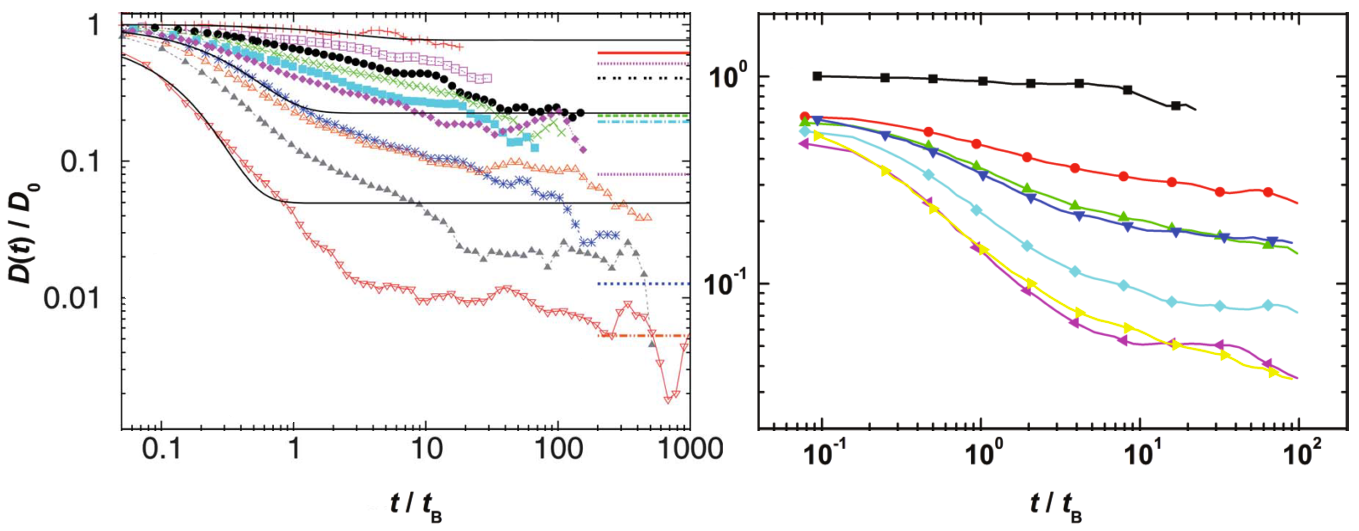
\includegraphics[width=14cm]{pics/ndc_exp.png}}
\caption{Top pictures: the mean square displacement in function of the time. Bottom picture: the normalized diffusion function in function of the time.
\\ Left: \small R. D. L. Hanes \etal, Soft Matter, \textbf{8}, 2714 (2012)\\ \normalfont Right: \small F. Evers \etal, Physical Review E, \textbf{88}, 022125 (2013)}
\label{msd ndc exp}
\end{figure}

The mean square displacement presents two variations of slope: at early times the behaviour is the same than for the system without external potential ($\varepsilon = 0$ in the picture from Evers \etal), the slope is equal to one, indicating a normal diffusion, at intermediate times the slope becomes lower (this happens earlier when the roughness is higher), the system is then said to have a subdiffusive behaviour, and for long times it returns to its initial value and follows again the slope of the $\varepsilon = 0$ curve.\\
The same kind of behaviour can be seen on the normalized diffusion coefficient: at small times the value is very close to one, meaning that the system follows a normal diffusive behaviour, then at intermediate times the value of $\nicefrac{D(t)}{D_0}$ decreases dramatically, finally at large times the system regains a diffusive behaviour, reaching a $D_{\infty}$ value.\\
These two physical quantities give precious information about the dynamics of the confined systems in function the time: at small times the system follows the behaviour of a non-confined fluid ($\left< \Delta r(t)^2\right>$ and $\nicefrac{D(t)}{D_0}$ have a diffusive behaviour), at intermediate times the system behave like it is trapped in the cages of the matrix and does not move as much as at earlier times (slopes of $\left< \Delta r(t)^2\right>$ and $\nicefrac{D(t)}{D_0}$ decrease), finally at large times, the system follows again a diffusive behaviour like at the beginning. This can be put in comparison with fig. \ref{relaxations}. Each of the observed regimes can be assigned to a relaxation regime: at early times the particles undergo a diffusive behaviour inside their local minima, then they start to hop from a minima to another until the system is under equilibrium, then they start to hop from a minima to another, which can be assimilated to a diffusive behaviour again.\jline

The Van Hove function is the probability density of finding a particle i at the position r at a time t, knowing that a particle j is at the origin at t=0. It is expressed as:

\begin{equation}
G(\Delta r,t) = \frac{1}{N} \left< \sum_{i=1}^N \sum_{j=1}^N \delta(r-r_i(t)+r_j(0)) \right>
\end{equation}

The Van Hove correlation function can then be split into two part: the distinct and the self parts:

\begin{align}
G_s(\Delta r,t) = &P(\Delta r,t) = \frac{1}{N} \left< \sum_{i=1}^N \delta(r-r_i(t)+r_i(0)) \right>\\
&G_d(\Delta r,t) = \frac{1}{N} \left< \sum_{j\neq i}^N \delta(r-r_j(t)+r_j(0)) \right>
\end{align}

The physical interpretation of the self part of the Van Hove function is the probability density of finding a particle i at the time t, knowing that this particle was at the origin at t=0. In other words, it the probability that this particle has moved of a distance r during the time t. The distinct part of the Van Hove function is the probability that a particle j different from i at a distance r at the time t, knowing that the particle i was a the origin at t=0.\\
The self part of the Van Hove function is often calculated during experiments or simulations because it give precious information about the dynamics of the system, as we can see in fig. \ref{spvhf exp}.

\begin{figure}[htbp]
\centering
\subfigure
{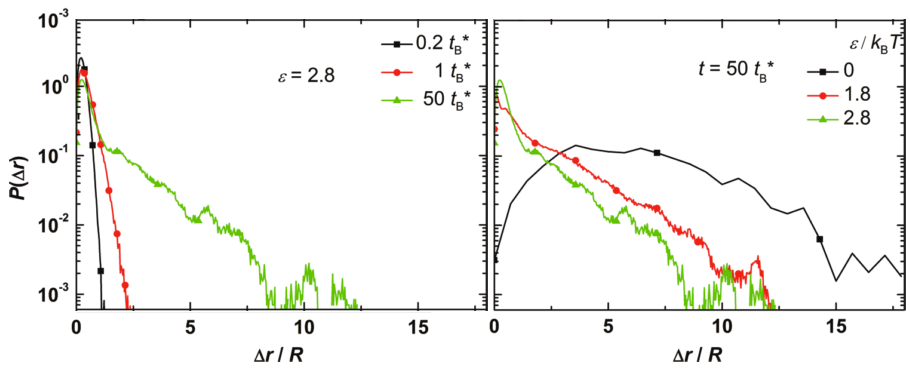
\includegraphics[width=14cm]{pics/spvhf_exp.png}}
\caption{Self part of the Van Hove function i-for different waiting times (left) and for different roughness (right).
\\F. Evers \etal, Physical Review E, \textbf{88}, 022125 (2013)}
\label{spvhf exp}
\end{figure}

From fig. \ref{spvhf exp}, we can see that the presence of a potential changes qualitatively the dynamics of the particles: the black curve at the right shows the self part of the Van Hove function without any potential and the green curve shows the same quantity with a roughness of 2.8. The behaviour is qualitatively different: when there is an external potential the particle explores less space, obviously because it remains trapped inside the minimas. Comparing the other curves we can say that, the less the waiting time, the less the particle can explore space, and the higher the roughness, the more the particle is trapped in the minima and the less it can move from its original position (this is clearly seen from the narrowing of the function for small times or high roughness).

\section{Theoretical models}
\label{theory}

This section will make a brief summary of the different models that have been developed in order to tackle the problem of the diffusion of particles in a disordered environment. The aim here is not to derive exactly every equation that makes the model, but simply to give a brief overview of the idea, problems and eventual results of these models.

\subsection{Random walk}
\label{random walk}

A simple way to see the diffusion in a disordered matrix is to model the dynamics of the particles by a random walk with constraints. This method is efficient when system where the particles are allowed to cross barriers (biological, magnetic systems...) Two models have emerged from this idea: the random trap model \cite{Haus1982} and the random barrier model \cite{Bernasconi1979,Jack2009}. The two models describe the diffusion from a one dimensional point of view, a simple model indeed, but precise enough to understand how diffusion works. The two models are not in concurrence but present a duality relation through their master operators.\jline

These two models are based on the assumption that the particle is Browninan, that is it has a random path through space. This type of behaviour is naturally very well described with a random walk.\jline

Consider a single particle hopping on a chain of sites. The particle on site $n$ may hop either to the right $n+1$, or to the left $n-1$. In the random trap model, each hop happen with a site-dependent rate $W_n$. Thus, the equation describing the dynamics of the random trap model is:

\begin{equation}
\frac{dp_n^T(t)}{dt}=W_{n+1}p_{n+1}^T(t)+W_{n-1}p_{n-1}^T(t)+2W_{n}p_{n}^T(t)
\end{equation}

In the random barrier model, the hopping rate is not site-dependent but barrier-dependent, that is dependent on the link between the sites:

\begin{equation}
\frac{dp_n^B(t)}{dt}=W_{n}\left[p_{n+1}^B(t)-p_{n}^B(t)\right]+W_{n-1}\left[p_{n-1}^B(t)-p_{n}^B(t)\right]
\end{equation}

The two models use the same set of rates $W_n$, then the fluctuation of the barrier model $j_n^B=W_n\left(p_N^B-P_{N+1}^B\right)$ and the rescaled probability density of the trap model $W_n p_N^T$ obey the same differential rules. It follows that when using the operator notation of $W_n$, the spectrum of eigenvalues of both models will be the same. This is called the trap-barrier duality. A simple way to understand it is to identify the regions between large barriers in the so-called model model with the deep traps in the trap model. This vision is not perfectly exact but has the advantage of clearly showing the kind of duality that links these two models. One can refer to the publication of Jack and Sollich about the barrier-trap duality \cite{Jack2007} for the exact derivation.\jline

RESULTS!!!!!!!!!!!!!!!!!!!!

\subsection{Monte-Carlo method}
\label{monte-carlo}

The Monte-Carlo method is a stochastic method that focuses on computing physical quantities by making a large number of calculations using random numbers, eventually averaging the results. This method is particularly suited in the kind of systems that were studied experimentally by Hanes \etal and Evers \etal (resumed in sec. \ref{exp}, which precisely made MC calculations to complete their work.\jline

The particle evolves in a computer-generated random potential. The simulations were made either by putting the particles randomly distributed in the potential energy surface (instantaneous quench of the system), or letting the particles relax and reach an equilibrium position (potential occupied following Boltzmann statistics). At each iteration a particle is randomly chosen, along with a direction. Then, the corresponding energy for a step in that direction is calculated from the particle's current position on the energy landscape. The move is accepted if the energy needed to make that step is low enough. It can also be put into a probability that depends on the energy of the step.\jline

\begin{figure}[htbp]
\centering
\subfigure
{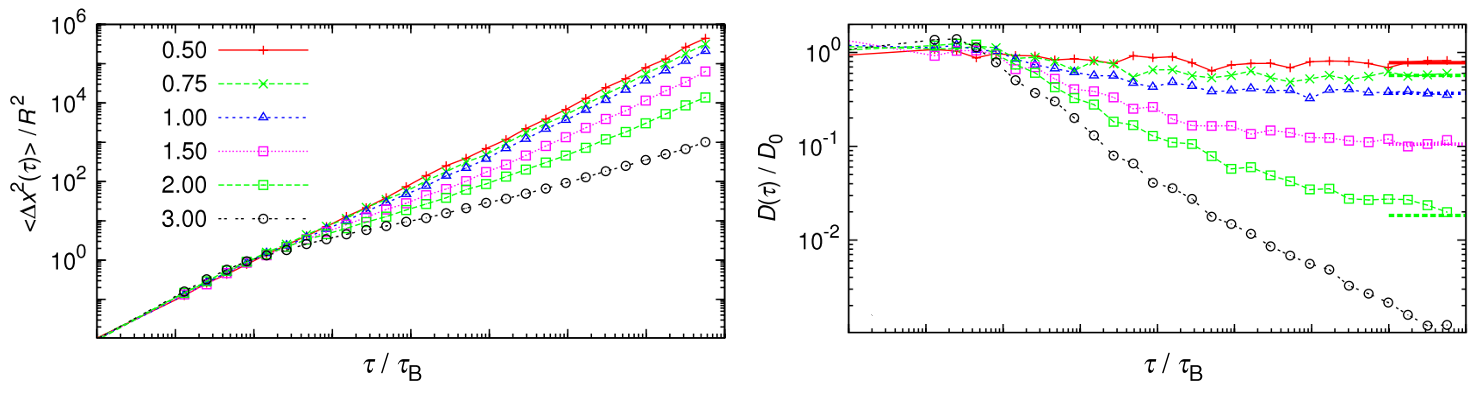
\includegraphics[width=14cm]{pics/msd_ndc_mc.png}}
\caption{}
\label{msd ndc mc}
\end{figure}


\subsection{Molecular Dynamics}

Molecular dynamics is one of the most used methods when making calculations about large systems of molecules or macromolecules. It is often used in drug design when it comes to model large proteins (often in addition with quantum mechanical methods, the so-called QM/MM). Molecular mechanics (MM), as expected, models the behaviour of molecular systems using the classical equations of motion (instead of quantum mechanical equations). This makes MM a very fast method by which thousands of atoms can be treated. It is also very adapted for thermodynamical and statistical systems, like for example liquids in confined matrices.\jline

A study from Chang \etal \cite{Chang2004} published in The American Physical Society presents a MM calculation of a binary mixture of hard spheres. One component is mobile and will undergo the dynamics, while the other component is fixed in space and time (similar to the QA mixture in sec. \ref{mct}). The algorithm calculates the velocity of each particle, and the new velocity after each collision.. Fig.\ref{msd ndc mm} shows the mean square displacement in function of time, and the normalized diffusion coefficient in function of the matrix/fluid ratio, as calculated with the MM algorithms.\jline

But before any analysis we have to define some quantities that are used in this publication. Since the matrix and the fluid are made of hard sphere particles, we can define $\sigma_mm$ as the matrix particle diameter, $\sigma_ff$ as the fluid particle diameter and $\sigma_{fm} = \sigma_{mf}$ as the typical paticle-matrix distance. The matrix and fluid volume fractions are defined as:

\begin{align}
\phi_{f/m} = \frac{\pi N \sigma_{ff/mm}^3}{6L^3}
\end{align}

\begin{figure}[htbp]
\centering
\subfigure
{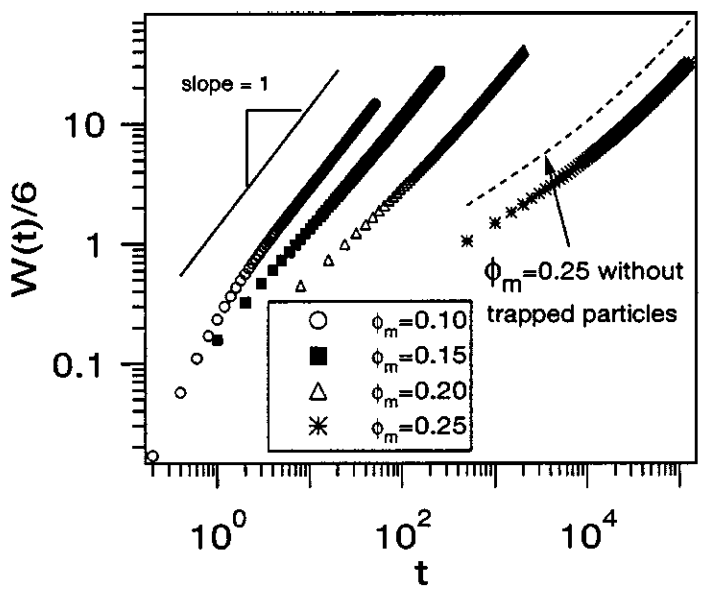
\includegraphics[width=7cm]{pics/msd_mm.png}}
\subfigure
{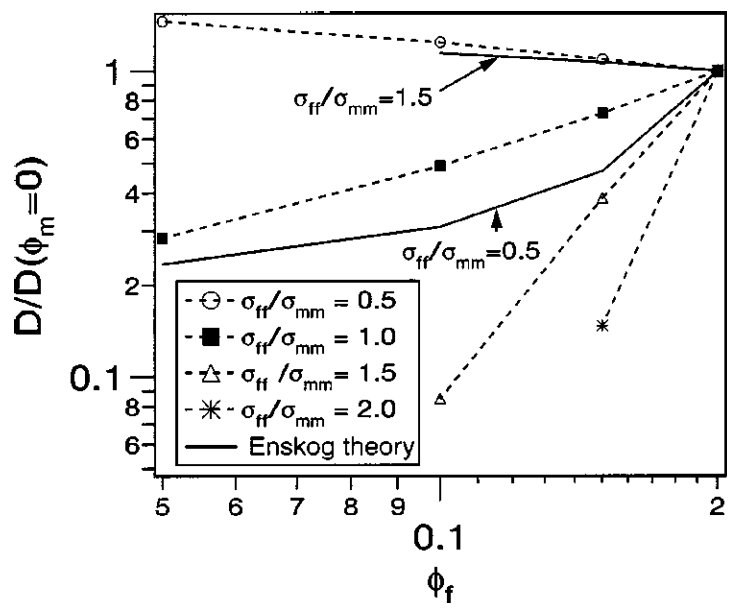
\includegraphics[width=7cm]{pics/ndc_mm.png}}
\caption{(left) Mean square displacement in function of time, the different curves show different matrix volume fractions $\phi_m$. (right) Normalized diffusion coefficient in function of the fluid volume fractions, the different curves show different $\nicefrac{\phi_f}{\phi_m}$ ratios.}
\label{msd ndc mm}
\end{figure}

As stated in sec. \ref{exp}, a system with a mean square displacement that follows a line with a slope equal to one has a diffusive behaviour. If the slope is lower than one, the system has a subdiffusive behaviour, and that is what happens when $\phi_m$ has a value around 0.25.\\

Fig. \ref{msd ndc mm} shows the normalized diffusion coefficient $D(t)/D_0$ as a function of $\phi_f$ for different values of $\sigma_{ff}$ for a fixed value of $\sigma_{mm}=1.0$. Therefore $\phi_m$ decreases as $\phi_f$ increases.\\
Something apparently strange happens: the curve has a qualitatively different behaviour when the ratio $\nicefrac{\phi_ff}{\phi_mm}$ changes. When $\sigma_{ff}$ is greater than $\sigma_{mm}$, the diffusion decreases as the size of the fluid particle increases. But when $\nicefrac{\sigma_{ff}}{\sigma_{mm}}<1.0$, the diffusion decreases when $\sigma_{ff}$ increases.\\
This can be understood as: when $\sigma_{ff}$ is greater that $\sigma_{mm}$, replacing a large fluid particle by several smaller immobile particles will create what is called a free volume. Free volume appears when matrix particles are so close to each other that some of the space is not available for fluid to flow in. This is why the diffusion decreases. \\
On the other hand, when $\sigma_{ff}$ is smaller than $\sigma_{mm}$, replacing several small fluid particles with a large matrix immobile one will tend to reduce the free space, and increasing the diffusion.

\subsection{Mode-Coupling theory}
\label{mct}

The Mode-Coupling Theory (MCT), developed by Wolfgang Gotze \etal \cite{Bengtzelius1984}, has emerged as one of the most accurate models for the dynamics of liquids, such that results from experiments or other simulations are often compared to MCT. The succes of MCT is its ability to reproduce reliably important phenomenas as the slowing down of the dynamics of a liquid when the temperature is decreases or when density increases.\jline

The MCT theory expresses the equation of motion, by projecting its terms on the slow modes of the system, resulting in a differential equation containing the correlation function (the function that connects the value of a quantity at time t with its value at time t+t', that physical quantity is usually the density and the density current) and the memory function (the function that "keeps" memory of all the trajectories of the system). The final MCT equation has the form:

\begin{equation}
\frac{\partial F(q,t)^2}{\partial^2}+\frac{q^2k_BT}{mS(q)}F(q,t)+\int_0^t d\tau K(q,t-\tau) \frac{\partial F(q,t)}{\partial \tau}=0
\end{equation}

Where $F(q,t)$ is the correlation function, $K(q,t)$ is the memory function and $S(q)$ is the structure factor (the correlation function between the physical quantity with itself at time t=0).\jline

The MCT has helped to make quality predictions of the liquid-glass transition on many bulk liquids, thus the idea emerged that MCT could be applied to systems presenting certain constraints. An extension of MCT has been developed for liquids confined between two flat parallel walls \cite{Lang2012} and for liquids confined in a disordered environment.\jline

The mode coupling theory describes the collective dynamics of liquids, instead of the dynamics of each single particle, as does the random walk for example. To simulate the presence of the disordered environment, the system is modeled by a binary mixture (called quenched-annealed mixture, QA mixture) in which one of the species would be immobilized (the quenched component), and the other component, the annealed component would follow the MCT dynamics (see fig. \ref{qa mixture}).

\begin{figure}[htbp]
\centering
\subfigure
{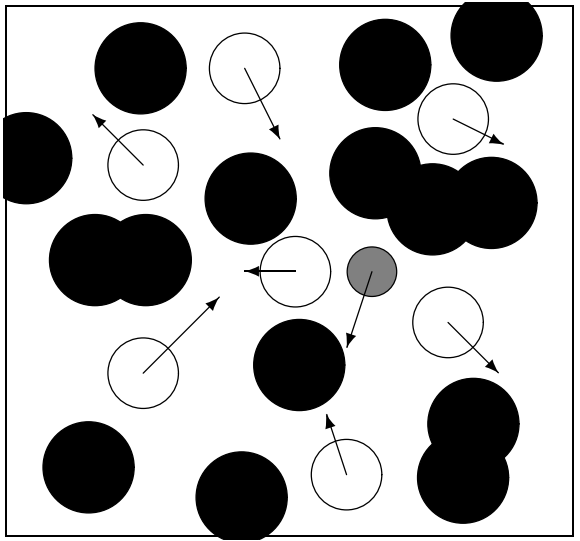
\includegraphics[width=7cm]{pics/qa_mixtures.png}}
\caption{}
\label{qa mixture}
\end{figure}

\newpage
\bibliographystyle{plain}
\bibliography{references}

\end{document}
